
\begin{frame}
    \frametitle{A Process's Gobal Memory Address Space}
    \begin{itemize}
        \item It is an extremely useful abstraction.
        \item But it's just an abstraction.
        \item And nowadays it's arguably an illusion.
    \end{itemize}
\end{frame}

\begin{frame}
    \frametitle{In Multithreaded Programs, The Illusion Breaks Down}
    \begin{itemize}
        \item In reality, data is shuffled between various memory heirarchy
              components.
        \item Per-core caches can greatly increase performance.
        \item But these caches can have inconsistent ``views'' of memory.

    \end{itemize}
\end{frame}

\begin{frame}
    \frametitle{Hardware Memory Model}
    \begin{itemize}
        \item A system's memory model is a contract between the system and the
              programmer.
        \item Informally, a memory model says how writes/stores on one processor
              are made visible to another processor.
    \end{itemize}
\end{frame}

\begin{frame}
    \frametitle{Java Slogan: ``Write Once Run Anywhere''}
    \begin{itemize}
        \item Java has been designed with strong portability guarantees between
              various hardware platforms.
        \item Java supports multithreaded programming.
        \item Java designers wanted to shield programmers from the subtleties
              hardware-specific memory models.
        \item So they made the Java Memory Model (JMM).
              \cite{manson2005java}\cite{pugh2004jsr133}\cite{manson2004jsr133}\cite{gosling2018jls11}
    \end{itemize}
\end{frame}

\begin{frame}
    \frametitle{The Java Memory Model (JMM)}
    \begin{itemize}
        \item A contract between a Java programmer and a Java platform.
        \item It says which executions of a program are legal.
        \item It gives programmers an (somewhat) intuitive model of concurrent
              programming.
        \item It constrains which program optimizations platform developers can
              implement.
        \item \dots
    \end{itemize}
\end{frame}

\begin{frame}
    \frametitle{The JMM Data Race Free Guarantee}
    \framesubtitle{The Formal JMM Result Discussed Here}
    Informally:
    \\~\\
    \begin{center}
        \Large
        \textit{If a program is data race free\\
        (a.k.a. ``correctly synchronized''),\\
        then the program's execution will\\
        be sequentially consistent.}
    \end{center}
\end{frame}

\begin{frame}
    \frametitle{Programmer Intuition of Sequentially Consistent Memory}
    \framesubtitle{Taken from \cite{adve1993designing}}
    \centering
    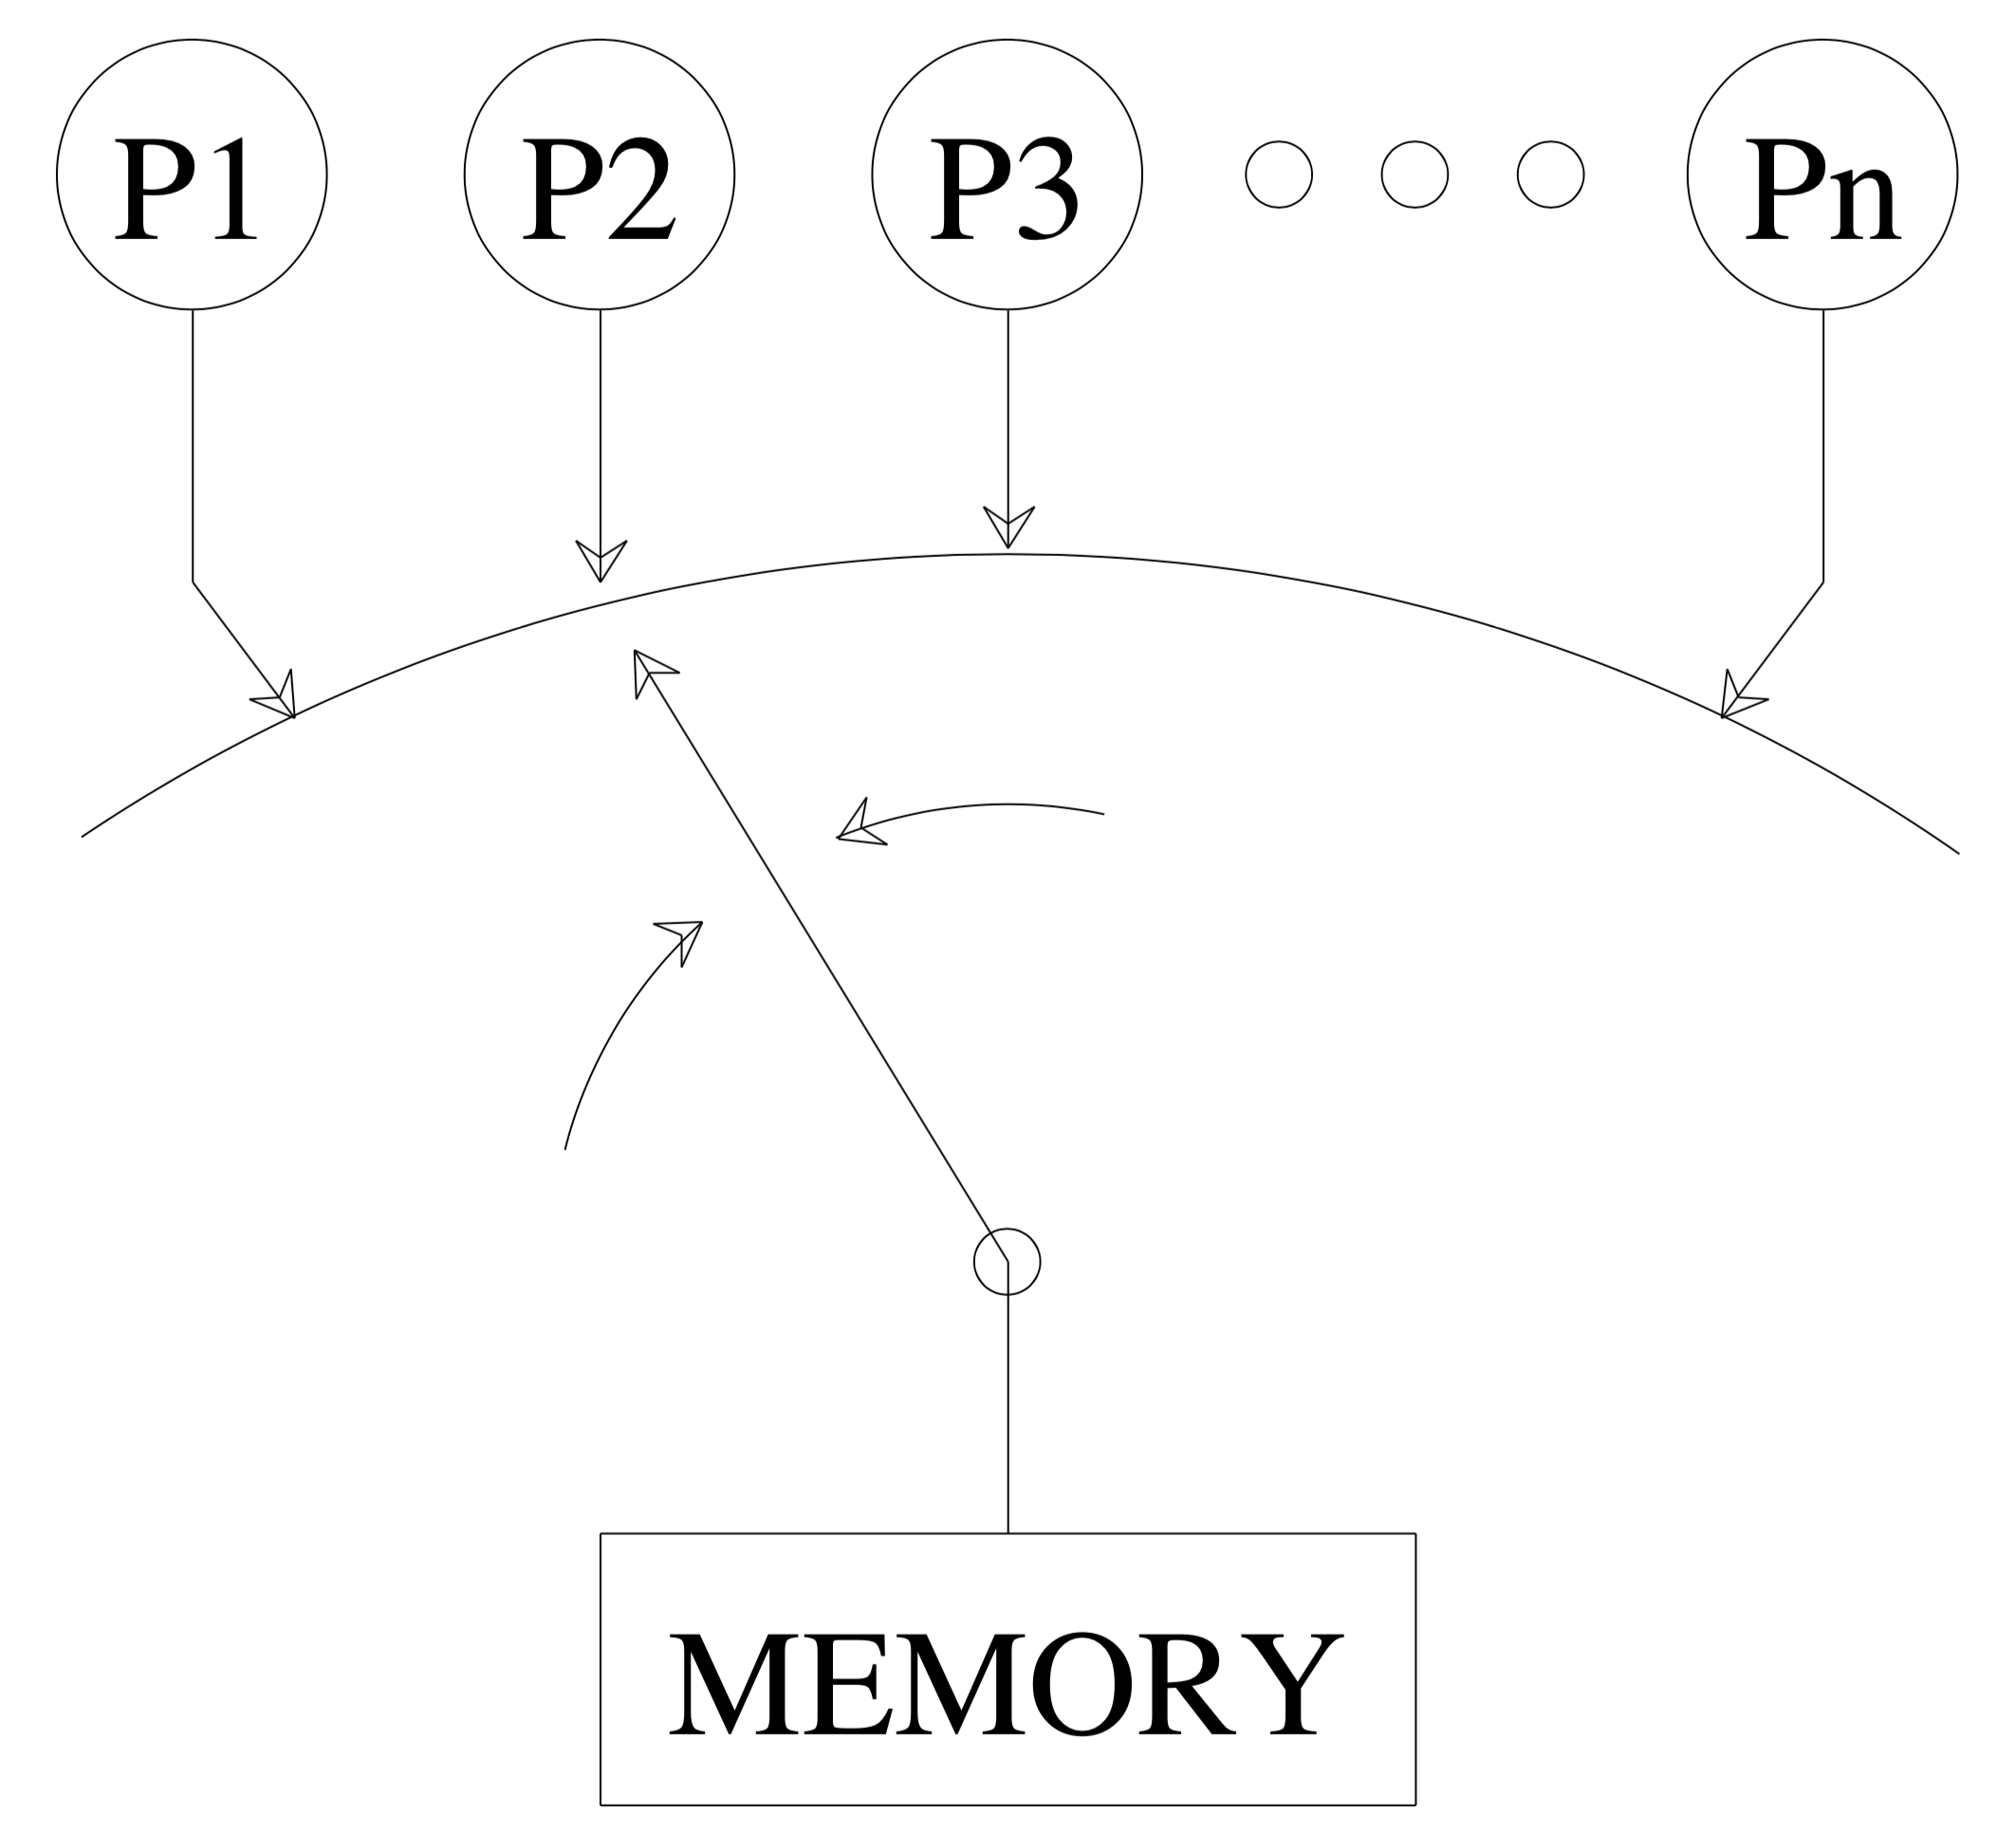
\includegraphics[width=\textwidth,height=0.85\textheight,keepaspectratio]{adve1995designing-figure_1_1.png}
\end{frame}

\begin{frame}
    \begin{itemize}
        \item Before we can formally define what we mean by sequential
              consistency, we need to pin down what we mean by execution.

        \item To precisely state and prove the aforementioned data race free
              guarantee, we need a bunch of definitions.

        \item We need a roadmap.
    \end{itemize}
\end{frame}

\begin{frame}
    \frametitle{JMM Definitions}
    \framesubtitle{A Roadmap to the JMM's Data Race Free Guarantee}
    \centering
    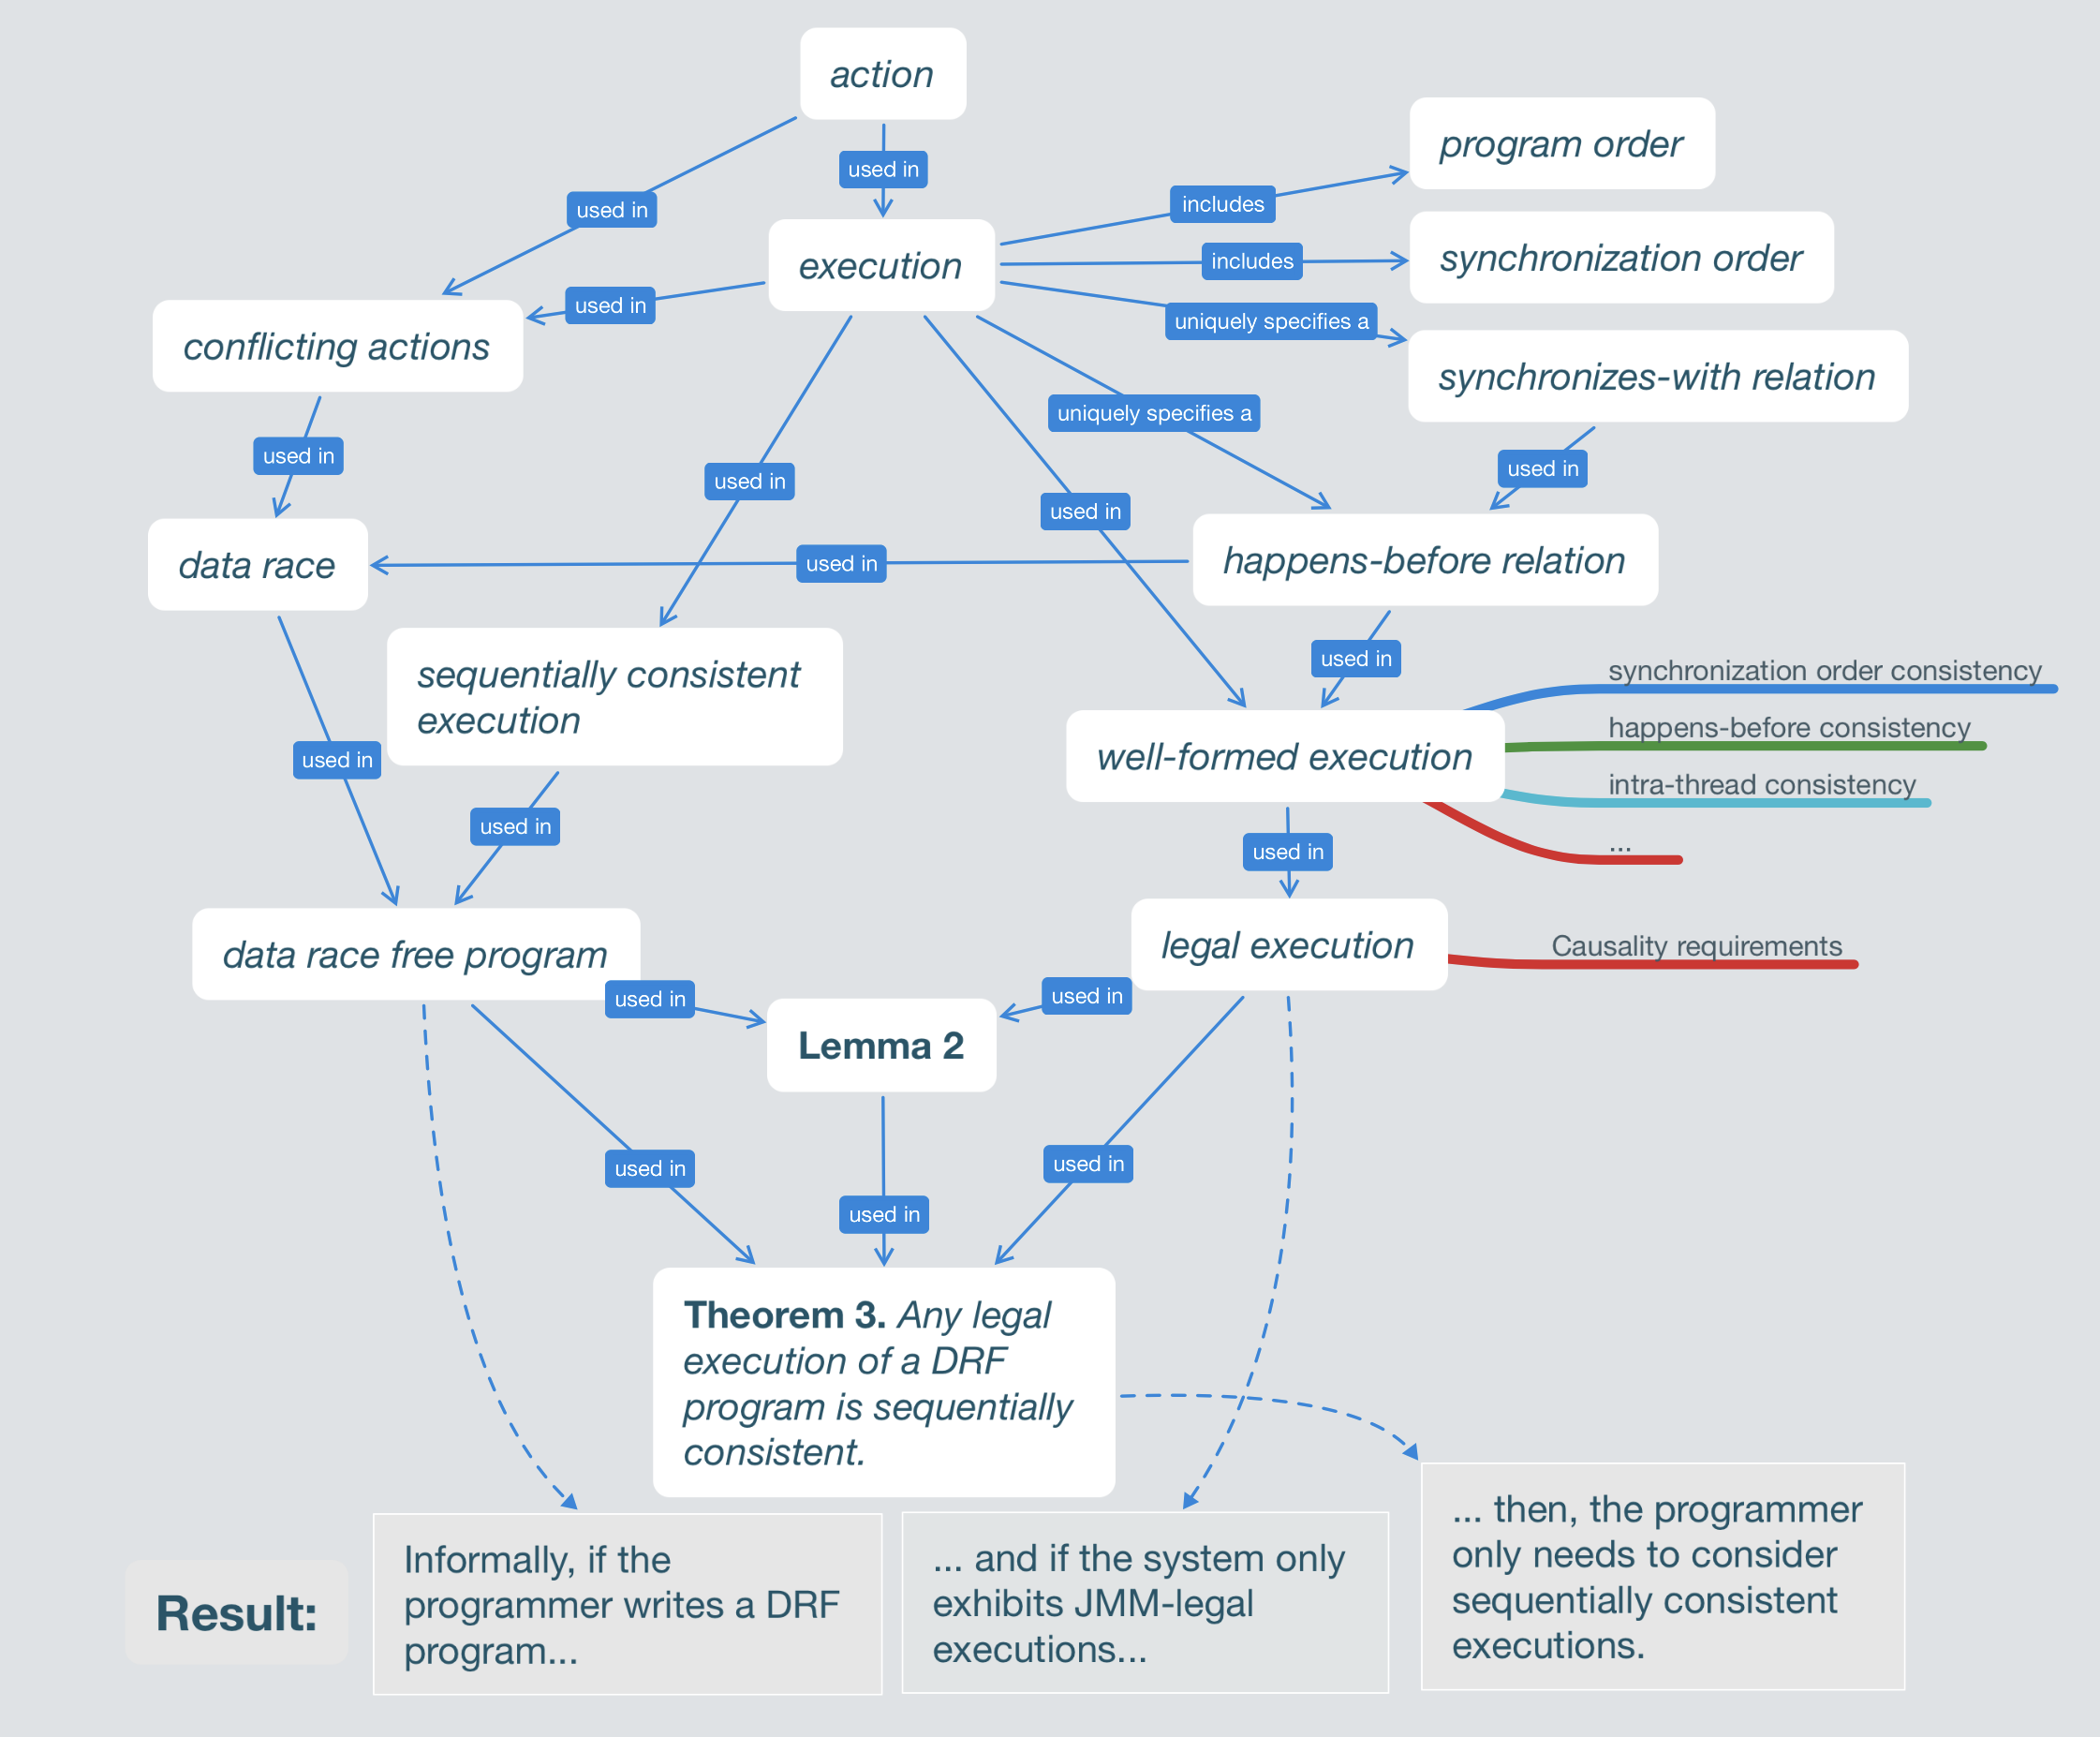
\includegraphics[width=\textwidth,height=0.85\textheight,keepaspectratio]{jmm_definitions_overview.png}
\end{frame}

\begin{frame}
    \frametitle{My Primary Sources}
    \begin{itemize}
        \item JSR 133, drafted Pugh et al. \cite{pugh2004jsr133}. Motivation and
              standards draft.
        \item Java Language Specification, Java SE 11 Edition \cite{gosling2018jls11}.
              The official standard.
        \item A POPL'05 paper by Manson, Pugh, and Adve \cite{manson2005java}:
              Motivations! Formalisms! Proofs!
        \item A Journal Paper by Aspinall and {\v{S}}ev{\v{c}}{\'i}k \cite{aspinall2007formalising}:
              Tweaked, fixed, and formalized the DRF guarantee with a proof
              assistant, Isabelle. We primarily follow this formalism.
    \end{itemize}
\end{frame}

\begin{frame}
    \frametitle{\textbf{Def.} Action}

    A memory related operation belonging to a particular thread; kinds:
    \begin{itemize}[itemsep=0.3em]
        \item volatile variable\footnote{The term variable is used throughout
              this discussion, but variable really means a Java object or
              a memory location.} read
        \item volatile variable write
        \item monitor lock
        \item monitor unlock
        \item normal variable read
        \item normal variable write
    \end{itemize}
\end{frame}

\begin{frame}
    \frametitle{\textbf{Def.} Execution}

    An execution is a 6-tuple $E = (A, P, \progorder, \synchorder, W, V)$, where

    \begin{itemize}[itemsep=0.3em]
        \item $A$, a set of actions
        \item $P$, a program
        \item $\progorder$, a partial order over $A$ called the \textit{program order}.
        \item $\synchorder$, a partial order over $A$ called the \textit{synchronization order}.
        \item $W$, the write-seen function between actions.
        \item $V$, the value-written function from actions to values.
    \end{itemize}

    \vspace{1.25em}

    \textbf{Key:} The JMM primarily exists to distinguish between legal/illegal
    executions.
\end{frame}

\begin{frame}
    \frametitle{\textbf{Def.} Synchronizes-With Order, $\synchwithorder$}

    \begin{itemize}
        \item Given an execution $E$, we can use its synchronization order,
              $\synchorder$, to derive $\synchwithorder$
    
        \item It is a more fine-grained partial order. It relates only those
              actions which directly synchronize with one another.

        \item \textbf{Def.} Let $a$ and $b$ be actions in $E$ such that
              $a \synchorder b$.
              \begin{itemize}[itemsep=0.3em,topsep=0.5em]
                  \item If $a$ unlocks a monitor which $b$ locks, or
                  \item if $a$ is a write and $b$ is a read of volatile variable
                        $v$,
              \end{itemize}
        then $a \synchwithorder b$.
    \end{itemize}
\end{frame}

\begin{frame}
    \frametitle{\textbf{Def.} Happens-Before Order, $\hborder$}

    \begin{itemize}
        \item We really only use $\synchwithorder$ as part of this next (very
              important) definition.

        \item The happens-before order is also derived from an execution $E$.

        \item \textbf{Def.} $\hborder$ is the transitive closure of the union of
              $\synchwithorder$ and $\progorder$.
    \end{itemize}
\end{frame}

\begin{frame}
    \frametitle{Defining Legal Executions}

    \begin{itemize}
        \item We can return to the JMM's primary responsibility: distinguishing
              legal from illegal executions.
        \item There are quite a few conditions required of a legal execution.
        \item These conditions are specified in two definitions:
        \begin{itemize}[itemsep=0.3em,topsep=0.5em]
            \item Well-formed execution (the ``simple stuff'')
            \item Legal execution (the ``harder stuff'')
        \end{itemize}
        \item As we will see, legality includes well-formedness.
    \end{itemize}
\end{frame}

\begin{frame}
    \frametitle{\textbf{Def.} Well-Formed Execution (informal)}
    \framesubtitle{The ``simple stuff''}
    \small
    We say that an execution $E = (A, P, \progorder, \synchorder, W, V)$ is
    well-formed if all nine of these conditions hold:

    \begin{itemize}[itemsep=0.3em]
        \item $A$ is finite.
        \item For each thread $t$, restricting $\progorder$ to $t$ is a total
              order.
        \item $\synchorder$ is a total order over synch (i.e. monitor/volatile)
              actions
        \item $\synchorder$ is consistent with $\progorder$.
        \item Reads to a particular variable only see writes to that variable.
        \item Proper locking on each monitor.
        \item $\progorder$ is intra-thread consistent.
        \item $\synchorder$ is synchronization-order consistent.
        \item $\hborder$ is happens-before consistent.
    \end{itemize}
\end{frame}

\begin{frame}
    \frametitle{\textbf{Def.} Intra-Thread Consistency}
    \framesubtitle{For Non-JMM Dynamic Semantics}

    Intra-thread consistency means that for each thread $t$, given all of the
    values that it read, the non-JMM parts of the Java language specification
    allow for the behavior observed in $\progorder \mid t$.
\end{frame}

\begin{frame}
    \frametitle{\textbf{Def.} Synchronization-Order Consistency}
    \framesubtitle{For Volatile Reads}

    For every volatile read $r$,
    \begin{itemize}[itemsep=0.3em]
        \item $r \not \synchorder W(r)$, and
        \item no write covers $W(r)$ in $\synchorder$,
              (i.e. $\not\exists w: W(r) \synchorder w \synchorder r$).
    \end{itemize}
\end{frame}

\begin{frame}
    \frametitle{\textbf{Def.} Happens-Before Consistency}
    \framesubtitle{For All Reads}

    \begin{itemize}
        \item This is similar to synchronization order consistency but w.r.t.
              all reads and the happens-before order.

        \item For every read $r$,
        \begin{itemize}[itemsep=0.3em]
            \item $r \not \hborder W(r)$
            \item $\not\exists w: W(r) \hborder w \hborder r$.
        \end{itemize}

        \item Notice that this doesn't say that a read must see a value which
              preceeds it in the $\hborder$. It just says that a read can't see
              writes covered in $\hborder$.
    \end{itemize}

\end{frame}

\begin{frame}
    \frametitle{\textbf{Def.} Legal Execution (Informal)}

    \begin{itemize}
        \item An execution is legal if it is well-formed and if there exists a
              sequence of increasing sets of \textit{committed actions} with
              \textit{justifying executions}.

        \item The definition is pretty technical.

        \item Motivation: Well-formed executions can have some very strange
              behaviors. In particular, ``out-of-thin-air'' values (i.e. values
              that have never been written to a variable) can be read.
    \end{itemize}
\end{frame}

\begin{frame}
    \frametitle{\textbf{Def.} Sequentially Consistent Execution}

    An execution is sequentially consistent if there is a exists a total order,
    $\totalorder$, such that:

    \begin{itemize}[itemsep=0.3em]
        \item $\totalorder$ is consistent with $\progorder$
        \item $\totalorder$ is consistent with $\synchorder$
        \item For any read $r$ of variable $v$, the execution reads the most
              recent write to $v$ in $\totalorder$.
    \end{itemize}
\end{frame}

\begin{frame}
    \frametitle{\textbf{Def.} Conflicting Actions}

    Two actions on the same variable in execution $E$ are conflicting if
    at least one of them is a write.
\end{frame}

\begin{frame}
    \frametitle{\textbf{Def.} Data Race}

    Two conflicting actions $a$ and $b$ form a \textit{data race} if neither
    $a \hborder b$ nor $b \hborder a$.
\end{frame}

\begin{frame}
    \frametitle{\textbf{Def.} Data Race Free (DRF) Program}

    \begin{itemize}
    \item Now we finally get to the point.

    \item A program is data-race-free if in all sequentially consistent
          executions, there are no data races.
    \end{itemize}
\end{frame}

\begin{frame}
    \frametitle{JMM Definitions}
    \framesubtitle{A Roadmap to the JMM's Data Race Free Guarantee}
    \centering
    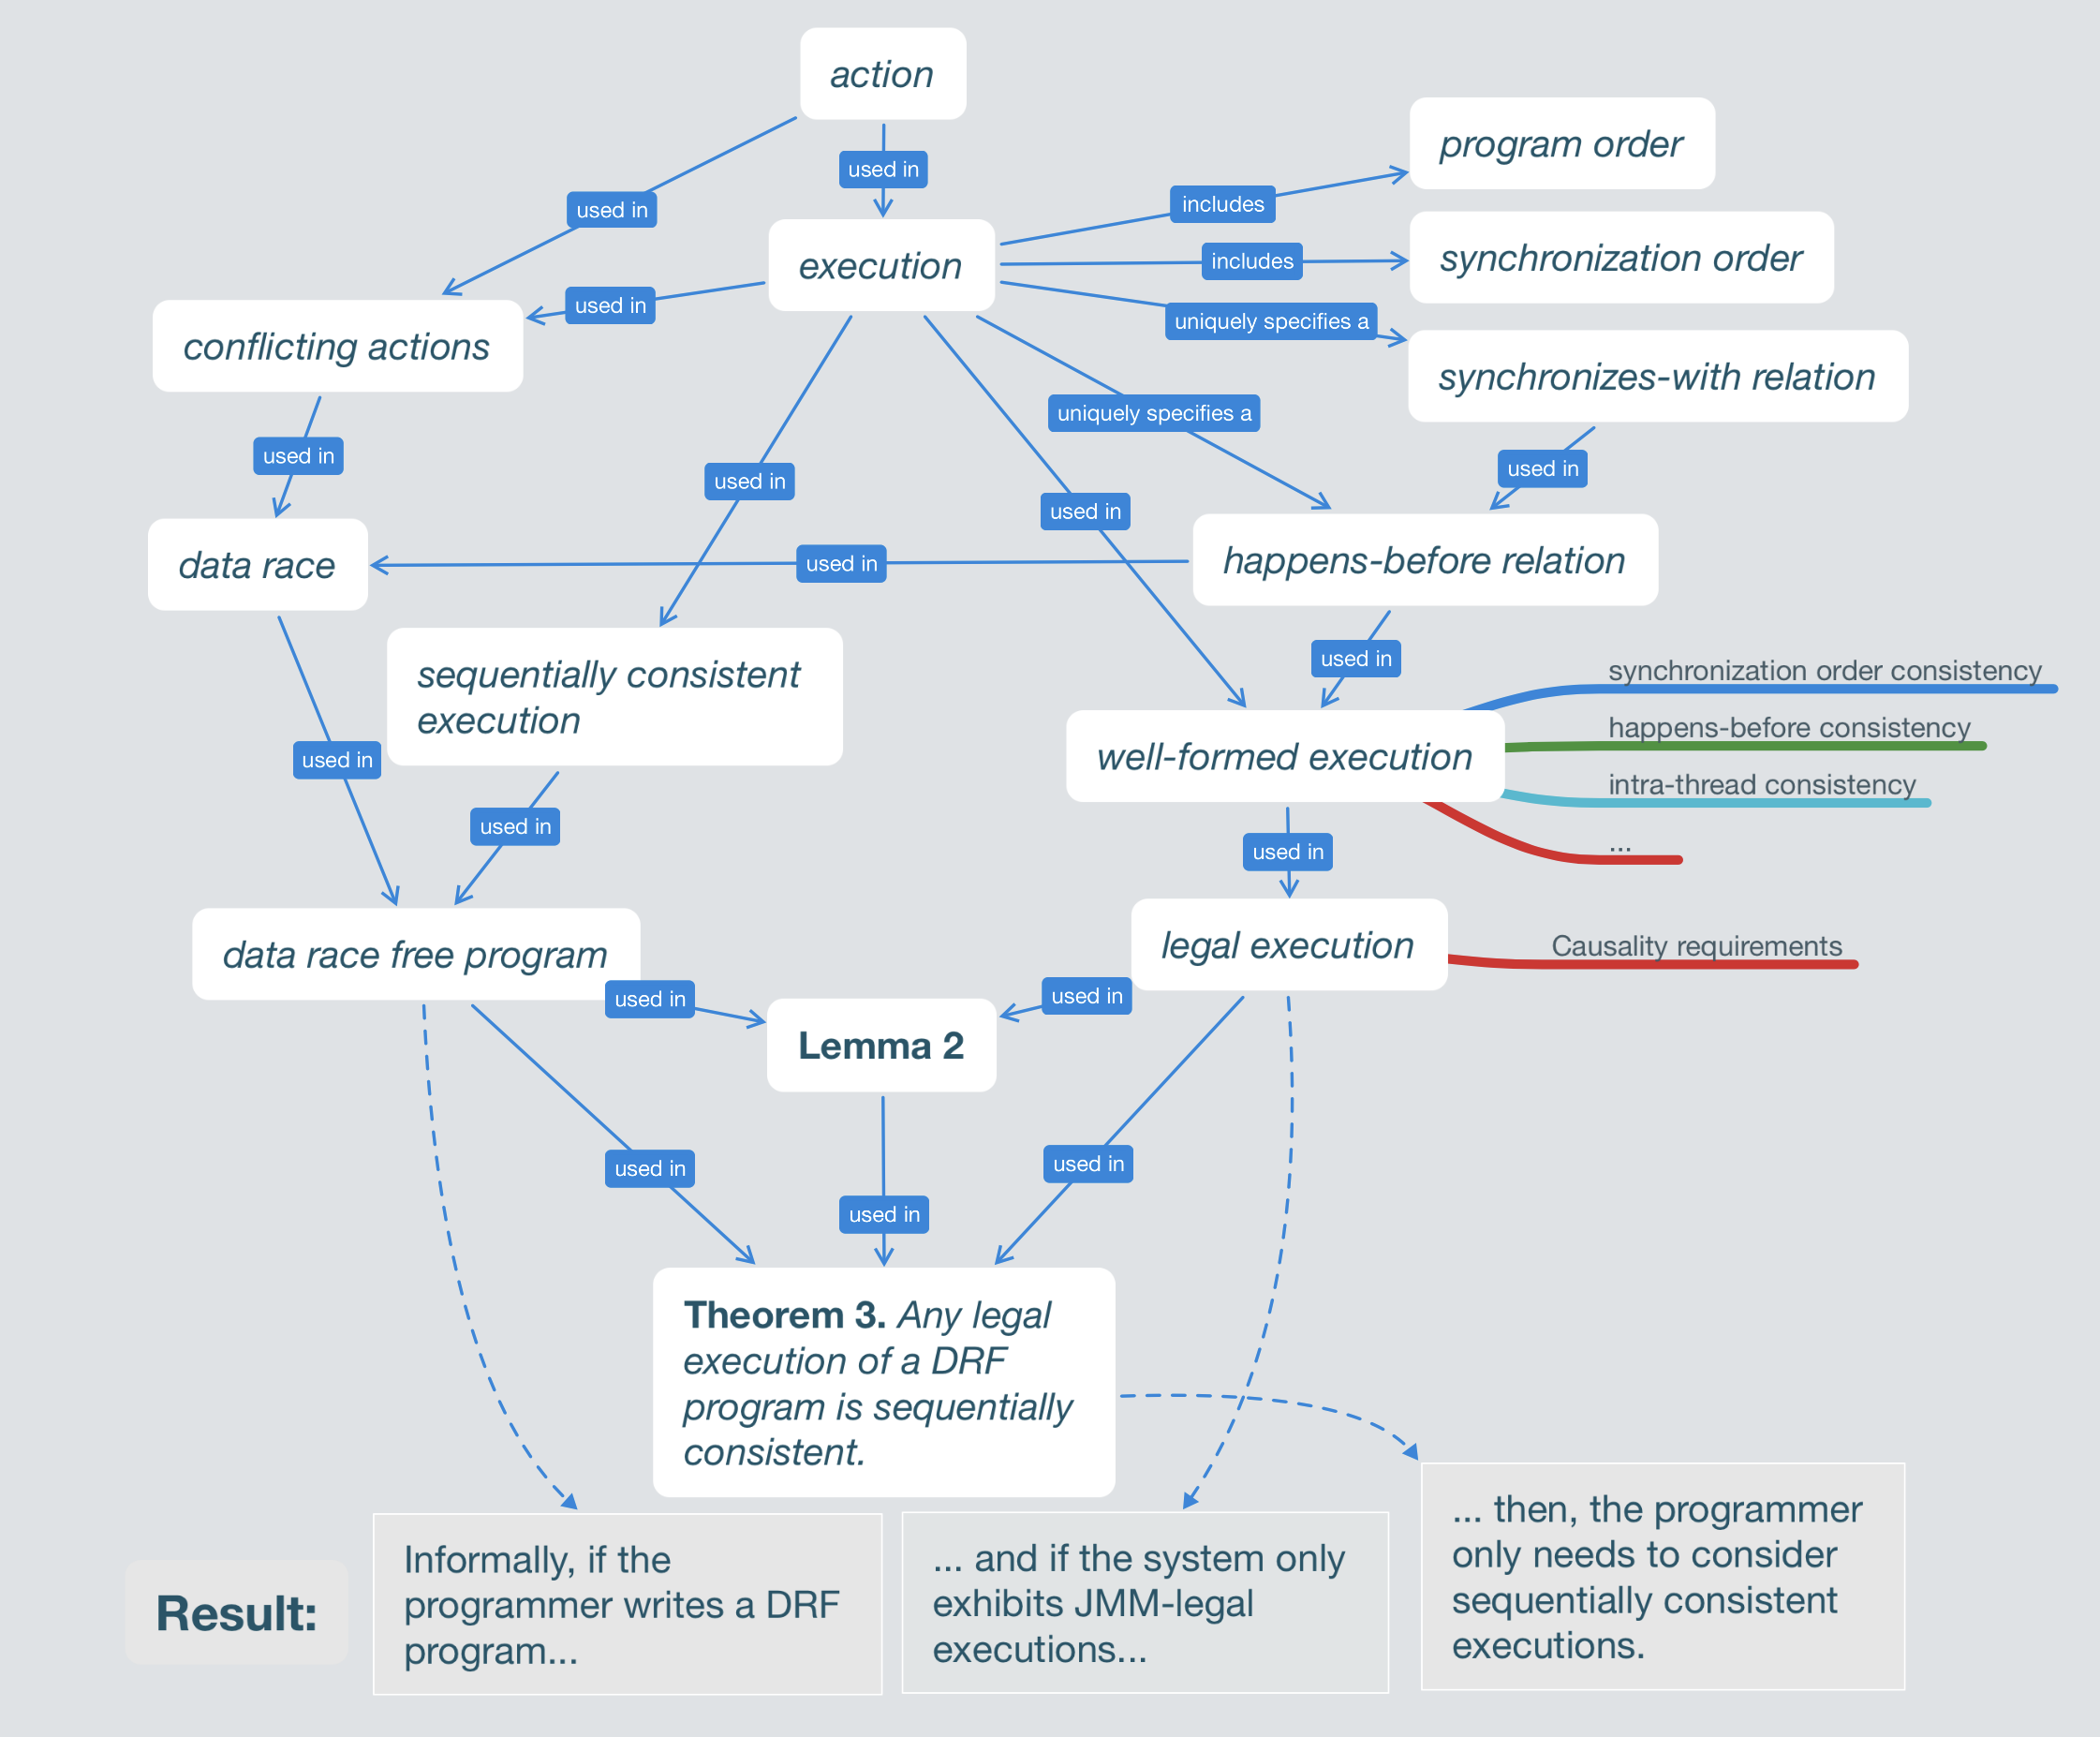
\includegraphics[width=\textwidth,height=0.85\textheight,keepaspectratio]{jmm_definitions_overview.png}
\end{frame}

\begin{frame}
    \frametitle{Theorem 3: JMM's DRF Guarantee}

    \centering
    \Large
    Any legal execution of a data-race-free program is sequentially consistent.
\end{frame}